\section{Protocol}
\label{sec:protocol}
This section presents the protocol and explains how it can improve the way vulnerability disclosures are completed for deterministically verifiable zero-day exploits.

\subsection{Scope}\label{subsec:scope}
For a specific type of vulnerability, some, to all of these concerns can be alleviated. The scope/applicability of the protocol is visualised in \cref{fig:protocol_scope}.
\begin{figure}[H]
    \centering
    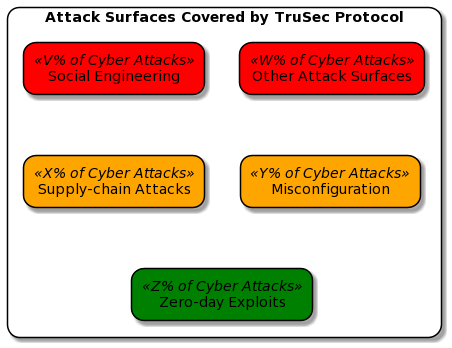
\includegraphics[width=0.50\textwidth]{images/plantuml/scope.png}
    \caption{(See notes) The proposed TruSec protocol is not suited to deal with social engineering attacks, nor is it ideal for misconfiguration exploits and/or supply-chain attacks. Instead, it is designed to increase the rate of discovery of zero-day exploits. Note, we acknowledge that attacks can be, and often are, a combination of the types.}
    \label{fig:protocol_scope}
\end{figure}

\noindent With this scope defined, one can look at how companies and ethical hackers interact according to the proposed protocol. This is visualised in \cref{fig:interaction}.

\begin{figure}[H]
    \centering
    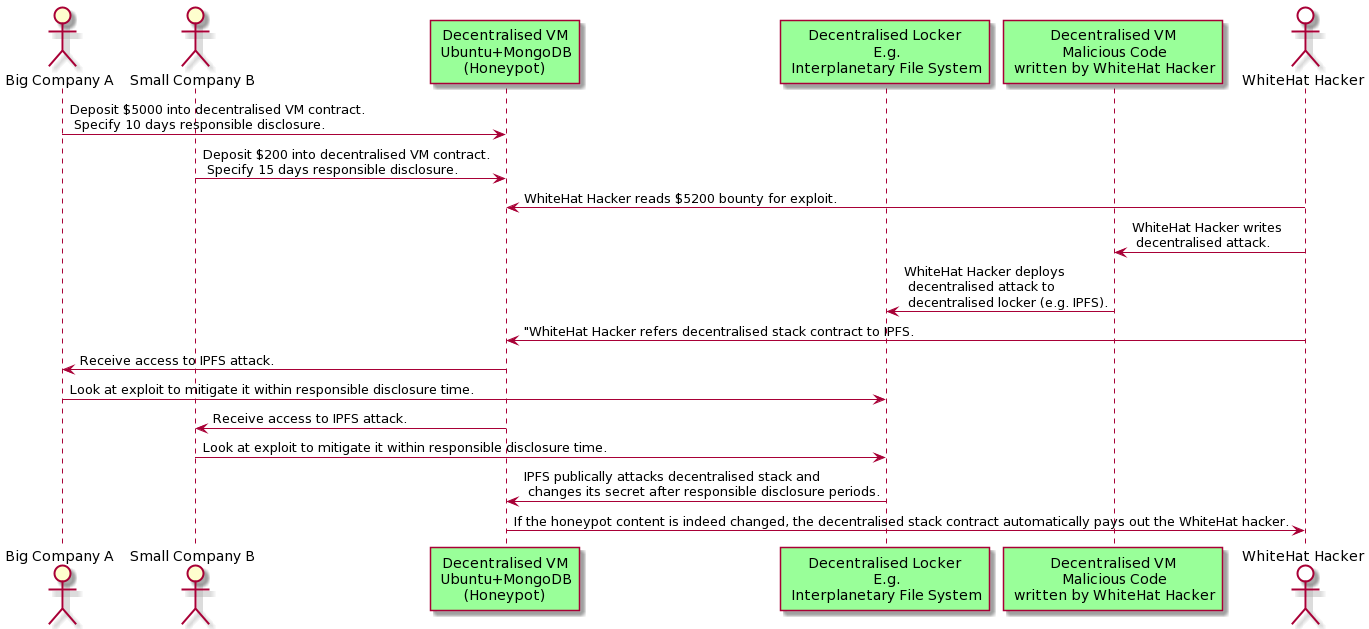
\includegraphics[width=1.0\textwidth]{images/plantuml/interaction.png}
    \caption{Visualisation of the interaction of the TruSec protocol. This is an ever-lasting cycle, where at the end of the process, companies can re-deploy the patched decentralised stack, and allocate new funds. Whitehat hackers can scan for new attacks.}
    \label{fig:interaction}
\end{figure}
\noindent So the basic idea is that companies can put their open source stacks on a decentralised virtual machine (honeypot), then collectively stake money on the stacks, such that everyone can see how much money says: \textit{the use of certain software packages/combinations is safe}. This enables companies, e.g. company $A$, to show their customers for example:

\textit{With us, your data is stored using MongoDB Version 5.1, \$314.159,- says it is uncompromised, and it's running on Ubuntu Server version 21.10, which has \$4.200.000,- staked on its security. This setup has a configuration with a security on which we staked \$9001,-. If any of these software packages get compromised by whitehat hackers, we will be the first to know.}

We believe that might be clear language that enables decision makers and customers interested in company $A$, to get an intuitive understanding on \textit{how secure} some (critical) segments of the company $A$ software is.

For the whitehat/ethical hackers, the advantages are clear; they know before they start their work how large their payout will be, and they get a direct payout upon completion (after the predetermined responsible disclosure period has ended).

Note. We are aware that the TruSec protocol does not provide a clear picture on the complete security of a system/company, since a chain is only as strong as its weakest link. Hence, if other attack surfaces, such as social engineering are used, companies can still get compromised, regardless of the amount they staked. Therefore, it is important that the numerical value of the amount staked on the zero-day exploit security level is not abused to convey a false sense of security by the staking companies to their customers. Nevertheless, we think for the zero-day-exploit the amounts staked on certain systems and/or configurations, may provide an improved insight.
\subsection{\Cref{fig:protocol_scope} notes}
With respect to \cref{fig:protocol_scope}, the following notes are made:
\begin{enumerate} 
    \item The orange attack types imply the proposed protocol is not designed to tackle these issues, nor does it provide full coverage (against economically rational, malicious agents) for these attack types. However,
    \begin{enumerate}
        \item The misconfiguration could be covered if companies upload their configurations into decentralised honeypots. These configurations would typically not benefit from the collaborative staking, as it is less likely that other companies happen to use the same configurations.
        \item Some of the supply chain attacks could be covered if the ethical hackers are able to propagate these supply chain exploits into the decentralised honeypot.
    \end{enumerate}
\end{enumerate}

\subsection{\Cref{fig:interaction} notes}
With respect to \cref{fig:interaction}, the following notes are made:
\begin{enumerate} 
    \item The attack written by the ethical hacker should be accessible on chain, such that everyone can verify that the attack indeed compromises the decentralised VM/honeypot. This is critical for the automatic payout.
    \item The decentralised locker is used to prevent malicious hackers to inspect/copy the attack before the responsible disclosure period is over.
    \item It would be better if the contract specifies the locker location, allowing the staking companies to actively check if an attack is found, instead of the attack reaching out to the honeypot. This is because the latter could attract unwanted attention. However, these are currently considered implementation details.
\end{enumerate}